\documentclass[12pt,a4paper,UTF8]{article}
\usepackage{ctex} % Chinese support
\usepackage{graphicx} % Insert images
\usepackage{listings} % Print source code
\usepackage{color} % Color support
\usepackage{booktabs} % Professional table support
\usepackage{pdflscape} % Landscape pages support in PDF
\usepackage{hyperref} % Hypertext links support for cross-referencing

% Customize hyperref format (it's set to no special format here)
\hypersetup{hidelinks}

% Declare directories to search for graphics files for graphicx
\graphicspath{{figures/}{logo/}}

% Define source code style for listings
\lstdefinestyle{c}{
  language=C,
  basicstyle=\ttfamily\footnotesize,
  keywordstyle=\bfseries\color[rgb]{0, 0, 1},
  identifierstyle=\color[rgb]{0.2, 0.2, 0},
  stringstyle=\color[rgb]{0.6, 0.1, 0.1},
  commentstyle=\itshape\color[rgb]{0.05, 0.5, 0.05},
  backgroundcolor=\color[gray]{0.95},
  numbers=left,
  numbersep=5pt,
  numberstyle=\color[gray]{0.6},
  breaklines=true
}

% Define new command for title page
\newcommand{\reporttitle}[2]{
  \LARGE\textsf{#1}\quad\underline{\makebox[12em]{#2}}
}
\newcommand{\reportinfo}[2]{
  \large\makebox[4em]{\textsf{#1}}\quad\underline{\makebox[18em]{#2}}
}

% The document begins here
\begin{document}
\begin{titlepage}
  \centering
  \vspace*{\fill}
  
\includegraphics[height=144pt]{nju-logo}\\[48pt]
  {\huge\textsf{课\ 程\ 实\ 验\ 报\ 告}}\\[48pt]
  \reporttitle{实验名称}{进程调度}\\[72pt]

  \reportinfo{课程名称}{操作系统}\\[8pt]
  \reportinfo{院\hspace{\fill}系}{计算机科学与技术系}\\[8pt]
  \reportinfo{学\hspace{\fill}号}{191220129}\\[8pt]
  \reportinfo{姓\hspace{\fill}名}{邢尚禹}\\[8pt]
  \reportinfo{邮\hspace{\fill}箱}{191220129@smail.nju.edu.cn}\\[8pt]
  \reportinfo{实验日期}{2021年4月}\\
  \vspace*{\fill}
\end{titlepage}

\tableofcontents
\newpage
\section{实验进度和批改注意事项}
已完成所有内容,包括选做。
\par 批改时希望能关注这一点:框架代码的bootloader\textbf{无法}在我的环境中正确运行(ubuntu20.04 + gcc 9.3),必须注释bootMain函数的以下两行(第16,17行):
\lstinputlisting[style=c]{boot.c}
\par 我猜想可能是由于gcc版本的问题,如果批改时不能正确运行,请将上述两行取消注释再尝试编译。
\par 另外,在kernel/irqHandle.c中有几个宏,可以通过定义和取消定义实现对不同内容的测试。
\begin{itemize}
	\item LOG:从serial输出一些调试信息,如执行系统调用,进程切换,阻塞和解除阻塞等;
	\item TEST\_MULTI\_IRQ:测试中断嵌套;
	\item TEST\_COMPETE\_DISPLAY:测试共享资源竞争相关内容。
\end{itemize}

\section{实验思路和过程}
\subsection{完成库函数}
直接调用syscall函数,通过宏选择系统调用类型,再传入参数即可。
\lstinputlisting[style=c]{syscall.c}
\par 另外,为调试方便,需要自己补充一些库函数。由于框架代码已给出了putChar函数,它可以将指定的字符从串口输出。由此可以封装自己的log函数和logint函数,供调试使用。
\lstinputlisting[style=c]{log.c}

\subsection{时钟中断处理}
在时钟中断到来时,要完成以下的处理:
\begin{itemize}
	\item 更新被阻塞的进程的状态;
	\item 更新当前进程的时间片使用情况,确定是否需要切换进程;
	\item 进程切换。
\end{itemize}
状态更新、确定是否需要切换进程可以这样实现:
\lstinputlisting[style=c]{timer_update.c}
\par 进程切换可以直接采用指导文档给出的代码。

\subsection{系统调用例程}
\subsubsection{fork}
fork需要实现以下内容:
\begin{itemize}
	\item 拷贝pcb信息和用户栈;
	\item 设置pcb中只与子进程相关的信息,如pid,内核栈指针,段寄存器等;
	\item 准备返回值,放入对应进程的pcb中的eax中。
\end{itemize}
\lstinputlisting[style=c]{fork.c}

\subsubsection{sleep}
\par 函数sleep的实现并不困难,只需要将当前状态设置为STATE\_BLOCKED,并设置sleepTime,再模拟时钟中断即可。注意要检查参数是否合法。
\lstinputlisting[style=c]{sleep.c}

\subsubsection{exit}
和sleep类似,只需要将当前状态设置为STATE\_DAED,并模拟时钟中断。
\lstinputlisting[style=c]{exit.c}

\section{实验结果}
\subsection{进程切换及相关系统调用}
kernel可以加载用户程序运行,并进行正确的进程切换、系统调用。运行结果如下:
\begin{figure}[htbp]
	\centering
	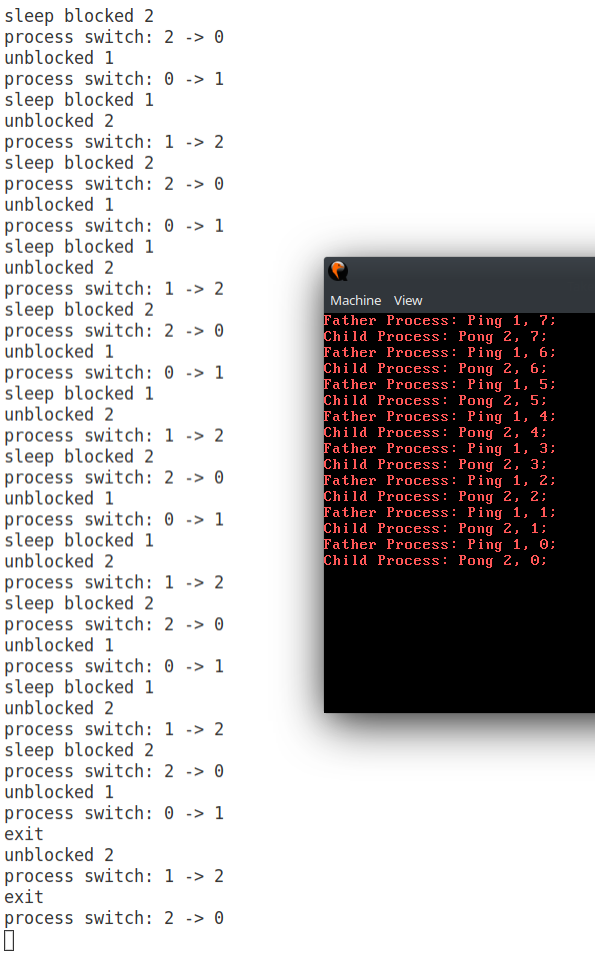
\includegraphics[width=0.9\textwidth]{switch}
	\caption{进程切换及相关系统调用运行结果}
\end{figure}

\newpage
\subsection{中断嵌套}
在fork中原始的用户栈复制代码中插入模拟时钟中断,实现中断的嵌套:
\lstinputlisting[style=c]{multi.c}
由于中断处理开销较大,如果在0x100000次循环中每次均插入一个时钟中断,运行非常缓慢。因此设置为每0x1000次插入一个时钟中断。运行结果如下:
\begin{figure}[htbp]
	\centering
	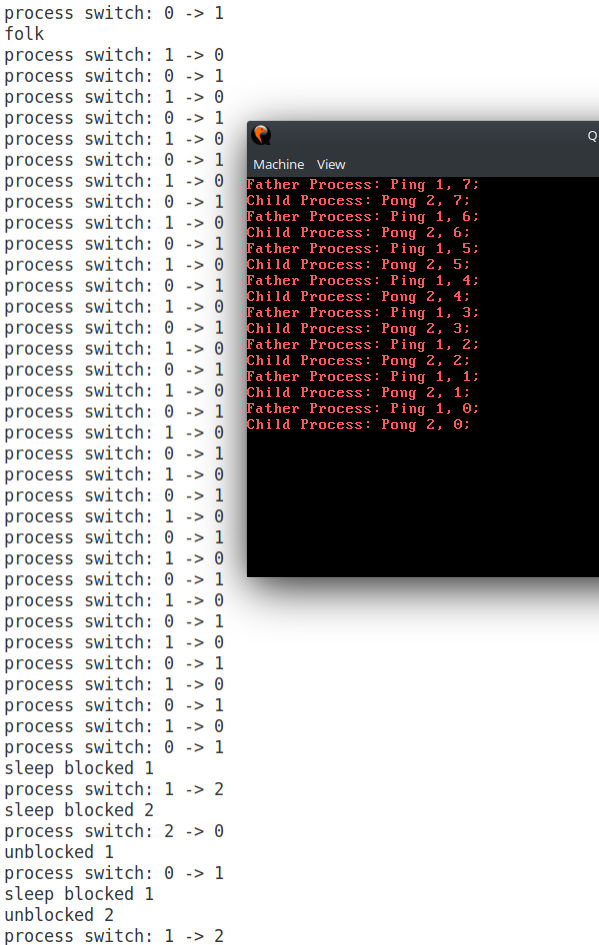
\includegraphics[width=0.9\textwidth]{multi}
	\caption{中断嵌套运行结果}
\end{figure}
\newpage
可见程序可以很好地支持中断的嵌套。

\subsection{共享资源竞争}
在syscallPrint函数中循环的最后添加一个模拟时钟中断,可以使多个syscallPrint函数并发执行。
\lstinputlisting[style=c]{compete.c}
运行结果如下:
\begin{figure}[htbp]
	\centering
	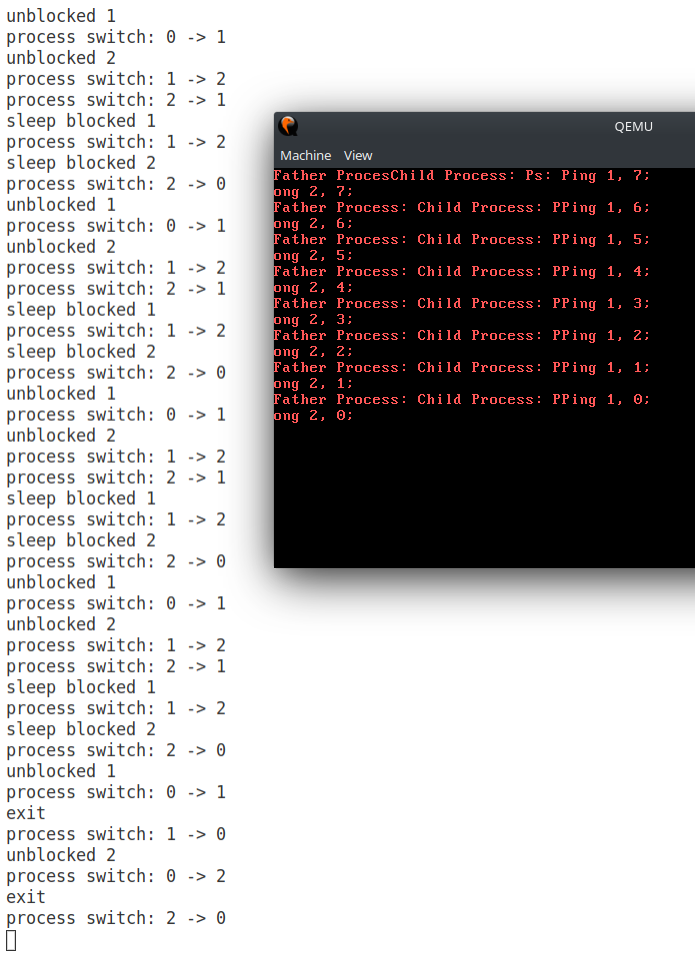
\includegraphics[width=0.9\textwidth]{compete}
	\caption{共享资源竞争运行结果}
\end{figure}
\newpage
可以看到,由于共享变量displayRow和displayCol被多个并发进程同时访问和修改,出现了打印上的问题。
\par 将相关代码反汇编,可以看到原本的执行流被int打断,再返回时,displayRow和displayCol被修改,就会出现错误。
\lstinputlisting[style=c]{print.s}

\section{问题与思考}
\begin{enumerate}
	\item 一开始直接使用框架代码给出的makefile进行编译并执行,但发现报错"boot block too large",于是根据实验0的相关指导将命令改为objcopy -S -j .text -O binary bootloader.elf bootloader.bin,即可正确完成编译。
	\item 在命令行中运行qemu-system-i386 os.img,窗口显示"no bootable device"。通过询问助教,得知原因可能是gcc版本问题。安装gcc6并编译可成功运行。另外,还有一个解决方案是加一个编译参数-fno-asynchronous-unwind-tables,经过尝试也可以成功。查询相关资料知,"This option determines whether unwind information is precise at an instruction boundary or at a call boundary. If -fno-asynchronous-unwind-tables is specified, the unwind table is precise at call boundaries only."新版本的gcc默认行为是"-fasynchronous-unwind-tables",而旧版的gcc默认"-fno-asynchronous-unwind-tables"。猜想unwind information的位置不同将影响加载过程,而qemu模拟的是老式的硬件,可能会产生不匹配。
	\item 在fork函数中拷贝pcb时,如果采用直接按位赋值的形式,即pcb[i] = pcb[current],则无法正常完成功能。这是由于pcb中有一个内核栈的数组,在按位赋值时只会复制指针(即浅拷贝),会使复制前后的指针指向同一个内存区域,造成错误。在使用C语言时,必须时刻注意类似的指针相关的问题,否则会出现严重的问题。
\end{enumerate}

\section{建议}
\begin{enumerate}
	\item 建议将官方的实验环境升级到20.04LTS版本,这样不容易产生gcc版本问题,可以节省很多时间;
	\item 既然一定会产生boot block too large的问题,建议直接将Makefile改成objcopy -S -j .text -O binary bootloader.elf bootloader.bin。
\end{enumerate}

\end{document}